\section{偏序格}
设\(\opair{L,\leq}\)是偏序集,\(\leq\)是\(L\)上的偏序关系,
\(L\)中的两个元素的上确界及下确界不一定存在.
例如,由哈斯图 \labelcref{figure:格论.偏序集1} 可知,
\(\{c,b\}\)无上确界,\(\{a,d\}\)无下确界.

\begin{figure}[htb]
%@see: 《离散数学》(邓辉文) P155 图5-1
	\centering
	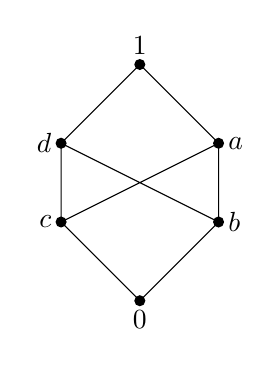
\begin{tikzpicture}
		\fill(0,0)circle(2pt);
		\fill(1,-1)circle(2pt);
		\fill(1,-2)circle(2pt);
		\fill(-1,-1)circle(2pt);
		\fill(-1,-2)circle(2pt);
		\fill(0,-3)circle(2pt);
		\draw(0,0)node[above]{$1$}
			--(1,-1)node[right]{$a$}
			--(1,-2)node[right]{$b$}
			--(0,-3)node[below]{$0$}
			--(-1,-2)node[left]{$c$}
			--(-1,-1)node[left]{$d$}--(0,0)
			(-1,-1)--(1,-2) (1,-1)--(-1,-2);
	\end{tikzpicture}
	\caption{}
	\label{figure:格论.偏序集1}
\end{figure}
